\chapter{Research Scope}

\section{Agenda}

What is the hypothesis of this research program?
What is the scope of the work?
What questions leading to experiments and observations emerge from the hypothesis and scope?

%%% \paragraph{Research Hypothesis}

%%% \paragraph{Research Questions}

	% \chapter{scope and objectives}

%%%	{\color{red} from document file: Main text V 4.2 (panel paper: part of "A hybrid SDN approach for Inter Domain Routing")}

\section{Initial Research Proposal}

\subsection{Anticipated Contributions}

Most proposals for improving routing in ISP networks involve disruptive changes of some kind - to the protocol itself, or to the network topology, or to router software. Such changes are at best risky, at worst impossible, within the context of existing operational networks. This proposal is quite different - it explores the limits of evolution within existing networks, decrying risky or disruptive changes. This thesis posits that existing network equipment and architectures have unexploited capabilities which can enable novel and far-reaching improvements to be made to existing networks and also provide an evolutionary path to a strategic new architecture.

The technical novelty of this proposal lies in the explicit selection of BGP \textit{as a southbound SDN protocol}. Implementations of network systems based on SDN and supporting BGP \textit{externally}, or as a \textit{northbound }interface (or east-west interface) exist, albeit in small number, however the positioning of BGP as a first class SDN protocol alongside OpenFlow, has had little if any attention within the field of SDN research.

The thesis anticipates a number of substantial contributions to research in the field:

\begin{itemize}
	\item the insight that there is currently a barrier to the application of SDN oriented academic insights within commercial ISP networks
	\item The application of an explicit hybridisation of centralised and distributed control in BGP networks
	\item bringing the benefits of an SDN approach and centralised control to the field of Internet routing
\end{itemize}

The concrete contributions anticipated from this work include:

\begin{itemize}
	\item \textit{A new architecture for production quality ISP networks}

	      The motivation for the new architecture is to enable intelligent centralised control over routing policy, with the goal of protecting network services from disruption caused by erroneous routing information arriving from other ISP networks, an additional goal being the improvement of service quality and resource utilisation. A further benefit of the proposal is that once fully deployed it enables further transformation in network elements, towards a disaggregated, vendor neutral, SDN capable system, with attendant commercial and technical advantages, including the promise of breaking the current logjam which prevents ISP networks from more fully benefiting from many other contributions from academic research.
	\item \textit{A migration strategy enabling non-disruptive deployment of the new architecture}

	      Unlike much other work this proposal is capable of incremental deployment within an existing network, with the ability to halt, reverse or temporarily disable in whole or in part the operation of the new system. This substantially mitigates the implementation risk and enables confidence and experience building over time. This makes it much more attractive for network operators.
	\item \textit{An implementation of the architecture}

	      The proposed practical implementation consists of an extensible software agent, deployed in a test network containing representative network equipment from leading vendors.

	      A practical implementation demonstrates the feasibility of the concept, and enables measurement and verification that real-world implementations can perform effectively. Since an important aspect of the thesis is the practical viability of the solution it is particularly important to demonstrate equivalence with existing systems in various domains.

	      The proposed practical implementation consists of an extensible software agent, deployed in a test network containing representative network equipment from leading vendors.
	\item \textit{An experimental framework for evaluating the function and performance of BGP routing systems}

	      Just as a practical implementation contributes to demonstrating the validity of the thesis itself, the validation of the implementation requires a capable test environment which adequately models relevant aspects of real networks and can monitor appropriate metrics. This is particularly important to validate the non-disruptive network migration capability which distinguishes this work. To enable this the test framework should be capable of generating realistic levels of both routing and user data traffic whilst simultaneously monitoring and correlating the system level behaviour in both control-plane and data-plane. The availability and ease-of-use of such a framework can contribute much to future research on various aspects of current and future networks.

	      Such a test framework is thus an essential complement to the implementation work, and will represent a significant contribution in its own right.
\end{itemize}

\subsection{Initial Problem Statement}

The problem statement flows directly from the propositions of the thesis, which are that, in the context of Internet core networks:

\begin{itemize}
	\item Existing approaches to policy specification and implementation of routing systems are sub-optimal
	\item Optimal routing requires a global view of network status
	\item Static and stateless policy languages are insufficiently powerful to specify optimal routing policy
	\item Existing network architectures and systems are capable of non-disruptive, evolutionary, enhancement to allow centralised oversight and control of routing policy and thus address the deficiencies mentioned above
\end{itemize}

The central problem is to evaluate whether such a system is practical. This leads to a number of specific sub-problems. These problems are classified as core, architecture and policy oriented:

\begin{itemize}
	\item Core
	      \begin{itemize}
		      \item How can a viable hybrid routing system be built?
		      \item Does it meet the basic requirements for operational deployment?
		      \item Does it demonstrate the improved capabilities which motivate the approach?
	      \end{itemize}
	\item Architecture
	      \begin{itemize}
		      \item Articulate the solution space - what are the options?
		      \item ‘Extrinsic’ aspects - treat policy agent as a black-box - how does it interact with the system?
		      \item ‘Intrinsic’ aspects - how do we build the agent?
		      \item Are there minor implementation changes or protocol extensions which could enable or improve the solutions
		      \item What limitations does the design impose?
		      \item What are the success criteria?
		      \item How can we test them?
	      \end{itemize}
	\item Policy
	      \begin{itemize}
		      \item Articulate exhaustively and explicitly real world policy
		      \item How can real world policy be expressed in a complete and unambiguous way
		      \item How can a system which implements such an explicit policy be built
		      \item Can such a system fall back to a basic policy implementation in the classical domain whilst supporting a centralised agent for optimal policy enforcement.
	      \end{itemize}
\end{itemize}

\subsubsection{Evaluation Objectives}

These research questions naturally feed into the evaluation approach, as follows:

\begin{itemize}
	\item Demonstrate the feasibility of building a hybrid routing system and show its viability.
	\item Characterise the performance of a range of solutions, including baseline reference systems which do not implement a hybrid architecture.
	\item Results should illuminate the respective merits of different approaches to building a hybrid routing system.
\end{itemize}
Another useful output of this work will be a test framework for evaluating functionality, performance and scalability of BGP routing systems.

\subsection{Architecture}

\subsubsection{Overview}

The solution proposed introduces a new architectural element called a Route Controller into a conventional BGP design. There may be one or more Route Controllers, and in a fully deployed scenario every border router in a BGP network will have an association to at least one Route Controller. Route Controllers communicate with border routers using the existing IP based BGP control plane, however that is implemented in the existing BGP network. The Route Controller both monitors and exerts control over each border router, using BMP to monitor routing state and BGP to control routing state. The BMP session between a border router and the Route Controller provides the Route Controller with a complete view of the external network as seen from the perspective of the border router. Figure 1 illustrates this architecture.

\begin{figure}
	\centering
	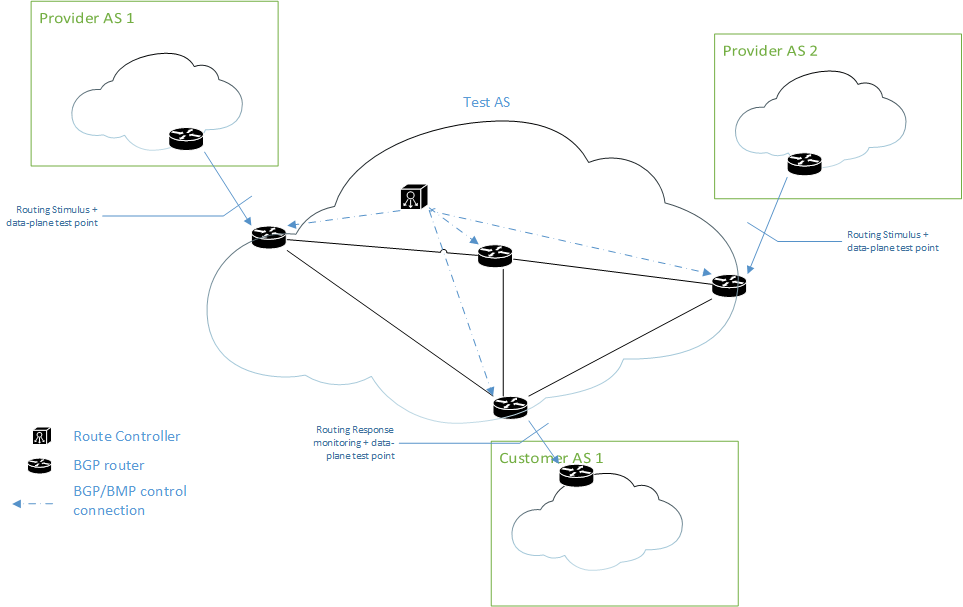
\includegraphics[width=0.5\linewidth]{images/simulated test network 1.1.png}
	\caption{Figure 1- Proposed Architecture}
	\label{fig:enter-label}
\end{figure}
% Figure 1- Proposed Architecture

\subsubsection{Route Controller Policy Agent}

The proposed Route Controller is presented above as a ‘black box’, which takes as input routing state information and produces as output routing decisions. However, the Route Controller only has value when the routing decisions it makes are better than those made by the existing classical routers. The topic of Routing Policy is too broad for any single work to address effectively; the intention in this thesis is to develop an instance of a Policy Agent for the Route Controller which exemplifies some of the possible attributes which the architecture enables. Some example important capabilities which will be explored in this work are:

\begin{itemize}
	\item Use of historical context to inform routing decisions
	\item Use of topological analysis to inform routing decisions
	\item Use of formal policy descriptions to inform routing decisions
\end{itemize}

%%% {\color{red} from document file: PIR / Thesis use cases}

\section{PIR / Thesis use cases}

\section{IDR applications}

It can be expected that the enabling impact of a programmable network will drive many more applications of immediate practical value as network operators awareness grows, but there are already plenty of examples which underline the value of the proposition in Internet routing applications, of which few are listed here:

\begin{itemize}
	\item enhanced re-routing based on fault location signalling
	\item route quality assessment before selection
	\item BGPSEC with acceptable performance
	\item Artemis style prefix hijack prevention
	\item route leak detection and mitigation (current PIR use case)
	\item route selection based on route stability (‘smart route-flap prevention’)
	\item smart load-balancing
	\item peer-specific preemptive route monitoring (‘active mode monitoring’)
	\item application of ML to routing
	\item use for AS internal security and diagnostic operations - e.g. traffic scrubbing, traffic monitoring, by injecting application specific route using flowSPEC
\end{itemize}
Similar challenges to traditional transit routing exist at IXP route-servers, and PIR offers the prospect of customised curated route selection based on diverse criteria. Indeed, many of the benefits of PIR are most applicable to routes exchanged at IXPs, and PIR also offers the prospect of mitigating some of the disadvantages of route servers as perceived by ISP members at IXPs.

Two of these applications are described now in a little more detail to demonstrate the immediate wider applicability of a PIR approach to IDR.

\subsection{enhanced re-routing based on fault location signalling}

A well known problem in BGP networks is the phenomenon described as ‘path hunting’ or path exploration, or ghost ....? See ....?. Path hunting is a process which takes place after a route failure and typically delays the process of converging on a new operable end-to-end route. In essence, path hunting is caused by short lived advertisements of unviable routes which also pass through the point of failure which triggered the first routing update. These transient unviable routes are generated by stale routes by routers situated close to the failure location.

There have been previous proposed solutions to this problem which either modify BGP protocol to signal fault location, or to propose systems which can infer route failure locations and make alternate route selections to those which are received as a result of path hunting. Whilst PIR could be put to use to implement those earlier proposals, this new design builds on that work whilst offering a more practical and readily deployable incremental approach to the same problem.

\subsubsection*{Methodology}

%%% <// this is more problem description than solution..

BGP routers are unaware of network topology, other than the restricted set of AS systems which are identified in routes received for routers closer to the route origin. After a link failure occurs in the currently announced path the eventually discovered working alternate path will likely differ significantly from the failed path at some location close to the origin, although that viable alternate may have to propagate though many of the same AS systems as those which lay on the failed path, and thus appear similar to both the original failed route, and also the subsequently propagated transient but unviable routes. Unfortunately however, the unviable routing messages which are received cannot easily be distinguished from the eventual first arriving good route. A further complication may arise in that there may be a complementary ‘storm’ of good routes as the new working routes are propagated at different rates through the intervening networks. An ancillary effect is a multiplication of the number of changing data points by the numbers of individual prefixes which were originally routed through the point of failure, some of which prefixes may eventually convergent to distinct routes after reconvergence and stabilisation is complete. But in this storm of routing information one piece of information is entirely missing, and not easily inferred, which is the actual point of failure, and even the fact that there \textit{is a} point of failure: route changes may as likely arise from added links as failed ones (the numbers of such events should of course balance out!). The reason for this dearth of information on failure locus is that the BGP failure message - ‘Withdraw’ - is most often replaced by a new route, and so either never propagated or only widely propagated very late in the path discovery process. Indeed, it is probable that if withdraw is received at all, for many routers it is the very last routing message to be received before a new viable alternate is received. The late arrival of withdraw is one reason that failure location signalling is hard to implement with much utility: the second is that the Withdraw message itself carries no information at all, other than the prefixes which can no longer be routed. So, when Withdraw is seen it is not possible to know where it originated, or even if its cause is a link failure, as opposed to a policy or configuration change.

%%% //>

\subsubsection{Variations on RCN}

Basic path exploration presents as updates to existing routes which are simple AS path extensions in which additional AS numbers are inserted in the previously received path. The failing AS is identifiable as the last unchanged AS in the path. At the failure locus the ghost routes are received from distinct peers, whilst at downstream points the replacement path announcements are combined within an announcement stream from a single peer, and mitigation options are different in the two cases. RCN proposed that, in the first case, withdrawal should be sent, before sending any further announcements.

It is worth analysing the objectives of RCN: ultimately, the goal is to rapidly restore service, however a subsidiary objective, which may also indirectly contribute to faster restoration, is to reduce transmission of ‘ghost routes’. In default BGP Service restoral depends on ‘bad’ routes being flushed out: ghost routes may directly delay this if they are still somehow preferred over the eventually selected stable alternate. Ghost routes can also delay restoral indirectly in two ways:

\subsection{route quality assessment before selection - ‘route curation’}

\subsubsection{Context}

For each routable prefix or group of prefixes an AS may receive routes from many sources: and in order to provide best service the AS selects just one route, but, lacking any stateful logic, the selection process is entirely reactive and depends only upon the instantaneous routing state. There is some justification for this approach: it is simple and predictable, and enables very rapid, locally decided, re-routing under topology change. However, the approach is hardly optimal: and almost every kind of routing failure or sub-optimality can be argued to result from this strategy. In a sense, that observation is trivial: if an outcome of a system is suboptimal, then the system can be improved.
But, the point is that making more refined decisions requires more complex logic, which may require a different processing approach. In essence, this is the heart of the PIR proposition.

This proposal is about an alternative operational strategy which aims to combine the advantages of simple distributed stateless route selection with the benefits of a more complex analytical approach. The approach is based on some simple reasonable assumptions about both network failure context, and about network routing threats. Concerning failures:

\begin{itemize}
	\item That rapid routing decisions are only required when responding to events which cause service failures.
	\item In many cases where an immediate response is required, the optimal alternate route selection is already available since long before the triggering event
\end{itemize}
Concerning routing threats

\begin{itemize}
	\item Adverse routing announcements are generally received and selected as ‘improvements’ over existing adequate routes.
	\item A potentially problematic exception to the first assumption is the case in which a preferred route source has already unwisely accepted an adverse route. However, even in this case a good, well established second-best candidate may be available.
	\item When the first assumption fails completely, i.e. no good alternate route is known at the local AS, then there is no sufficient AS response which can mitigate the problem
\end{itemize}
If these assumptions hold then a simple AS level behaviour exists which can improve network service by protecting against failures with rapid responses whilst applying more intensive analysis to new routes and thus enabling adverse routes to be rejected.

The AS behaviour required is this:

\textbf{Definition of Curated Route} For every received route an arbitrarily intensive analysis can be executed, and an aggregate preference calculated - this is similar to local preference, and it is likely that local preference attribute could be used to implement the strategy in a classical BGP network. Once a route has been analysed and scored it is made available for unrestricted selection - such routes are called ‘curated’ routes. As updates to existing routes are received from peers the curated attribute may be revised: depending on many factors the new route might be temporarily accepted into the curated list, possibly with a lower initial preference, or excluded until fully validated. The entire set of curated routes corresponds to an extended, AS wide, ADJ-RIB-OUT, such as might be implemented for ADDPATH.

\textbf{Application of Curated Routes}

At an AS level the principle is simple: whenever a curated route is available for a prefix it should be selected and announced: potentially, different curated routes could be announced to different peers, for business/policy/traffic engineering reasons. In one interpretation all curated routes should be immediately usable, e.g. a full operational MPLS path to the prefix via the originating external peer is available from any ingress ASBR. This interpretation would allow granular unrestricted selection between diverse routes within the AS.

\textbf{Curated Routes Impact on Route Selection}

The curation principle is simple: for all route selection, curated routes are selected in preference to non-curated ones, based on relative preference in all cases.

In practice this may be as simple as defining all directly received routes to have a local preference greater than some minimum, so that all curated routes are preferred. A refinement for this principle would be to allow specific border routers to assign ‘curated’ level preference to specific selected directly received external peer routes. The operational objective is defined at the AS level is simple, but the implementation detail in a classical AS is subject to design - not all curated routes are necessarily distributed to every border router, and various methods of distribution can be considered. an important aspect of a concrete implementation architecture is the decision about which curated routes to distribute, and to which border routers.

\section{Other BGP applications}

\subsection{Data centre}

BGP is already widely used in data-centre contexts, both multi-tenant (‘cloud’) and single tenant/enterprise. PIR techniques can easily be applied here too, for example for management of internal route selection security policy, or implementation of application specific route optimisation. BGP flowspec can easily be used to provision application specific routes in the dataplane, but the risk of complex and frequently updated router configurations are a disincentive to such innovation. Using an overlay controller based on PIR would enable such innovation in a controlled and fail-safe way. PIR could be used in conjunction with automatic configuration management systems to evaluate routing optimisation designs.

Application specific traffic routing is already widely used in enterprise settings, but in most cases the implementation requires customised hardware (middle-boxes). A programmable BGP controller using BGP and especially BGP flowspec could replace many such complex systems and unify the routing design into a simpler, more flexible, SDN style network fabric.

PIR could also find application in multi-tenant BGP environments, where it could be used in conjunction with

\subsection{Ethernet VPN (EVPN)}

EVPN is rapidly emerging as a useful technology for large scale (non-internet) service provider networks, e.g. Sky Broadband deployment in Italy (cite UKNOF London 2019).

Without a controller capability it is as difficult to manage EVPN systems as it is the global internet, i.e. the distributed static policy configuration approach does not allow complex or granular policies to be applied. PIR is a natural candidate for enhancing the manageability of such networks.
